% Shared network for the BFS, DFS, and traversal-lab notebooks.
% Run make here to rebuild the PDF and the notebook's SVG.
\documentclass[11pt,tikz,border=8pt]{standalone}
\usepackage{fontspec}
\IfFontExistsTF{Helvetica Neue}{
  \setsansfont{Helvetica Neue}[BoldFont={Helvetica Neue Medium}]
}{
  \setsansfont{TeX Gyre Heros}
}
\renewcommand{\familydefault}{\sfdefault}
\usetikzlibrary{arrows.meta}

\definecolor{graphink}{HTML}{303030}
\definecolor{graphred}{HTML}{EF4136}
\pagecolor{white}
\tikzset{
  graph vertex/.style={
    circle, draw=graphred, fill=white, line width=1.05pt,
    minimum size=8mm, inner sep=0pt, outer sep=0pt,
    text=graphink, font=\fontsize{12}{14}\selectfont\bfseries
  },
  graph edge/.style={
    draw=graphink, line width=0.85pt, line cap=round,
    -{Stealth[length=2.6mm,width=1.8mm]}, shorten >=1pt
  },
  edge weight/.style={
    midway, text=graphink, inner sep=1.5pt,
    font=\fontsize{11}{13}\selectfont
  }
}

\begin{document}
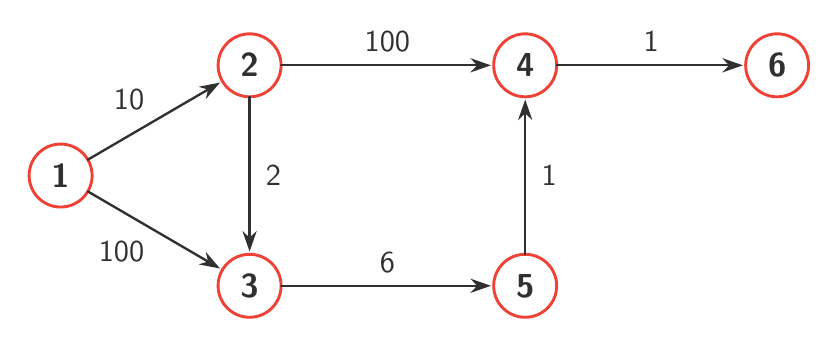
\begin{tikzpicture}[x=1cm,y=1cm]
  % Retain the lab layout: two rows and a starting vertex between them.
  \node[graph vertex] (v1) at (0.0,1.4) {1};
  \node[graph vertex] (v2) at (2.4,2.8) {2};
  \node[graph vertex] (v3) at (2.4,0.0) {3};
  \node[graph vertex] (v4) at (5.9,2.8) {4};
  \node[graph vertex] (v5) at (5.9,0.0) {5};
  \node[graph vertex] (v6) at (9.1,2.8) {6};

  % Edge directions and weights match ../data/SimpleGraph.txt.
  % Labels sit beside the edges; arrow tips stop short of the vertex borders.
  \draw[graph edge] (v1) -- node[edge weight,above left=2pt] {10} (v2);
  \draw[graph edge] (v1) -- node[edge weight,below left=2pt] {100} (v3);
  \draw[graph edge] (v2) -- node[edge weight,right=4pt] {2} (v3);
  \draw[graph edge] (v2) -- node[edge weight,above=3pt] {100} (v4);
  \draw[graph edge] (v3) -- node[edge weight,above=3pt] {6} (v5);
  \draw[graph edge] (v4) -- node[edge weight,above=3pt] {1} (v6);
  \draw[graph edge] (v5) -- node[edge weight,right=4pt] {1} (v4);
\end{tikzpicture}
\end{document}
